%نام و نام خانوادگی:
%شماره دانشجویی: 
\مسئله{}
چگونه می‌توان کیفیت طراحی یک نرم‌افزار را ارزیابی کرد؟


\پاسخ{

در بررسی کیفیت طراحی نرم‌افزار باید توجه داشته باشیم که بررسی کیفیت هر چیزی به صورت مطلق کار سختی‌ است و اینکار معمولا به صورت نسبی انجام می‌شود. و همچنین باید توجه داشت که کیفیت طراحی یک نرم‌افزار بیش از هر چیز مربوط به بررسی این است که طراحی ما نیازمندی‌های تعریف شده در آنالیز و به طور کلی تمامی نیاز‌های مشتری را پاسخ دهد.

برای بررسی کیفیت باید تصورات خودمان از کیفیت را به مواردی که قابلیت اندازه‌گیری و پیش‌بینی داشته باشند تبدیل کنیم.
همچنین حواسمان هست که دو دسته نیازمندی‌های عملکردی و غیرعملکردی داریم.

برای بررسی آنکه این دو دسته نیازمندی به خوبی پاسخ داده می‌شوند یا نه نیاز است تا طراحی خوانا باشد و توضیح قابل فهمی برای افرادی که مسئول نوشتن کد و همچنین تست و نگهداری از کد هستند داشته باشد. همچنین طراحی باید یک تصویر کامل از نرم‌افزار، داده‌ها و دامنه‌های عملکردی و رفتاری آن از دیدگاه پیاده‌سازی داشته باشد.

\begin{figure}[!ht]
	\centering
	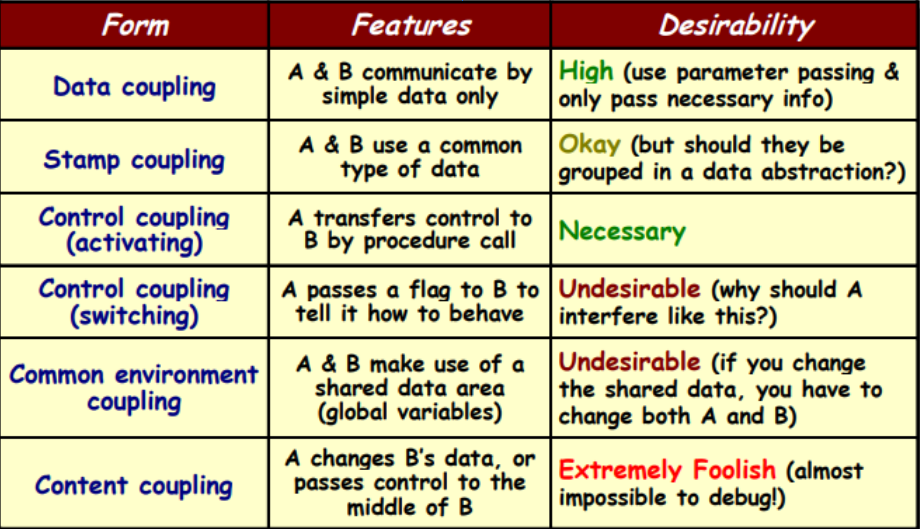
\includegraphics[scale=0.4]{figs/coupling.png}
	\caption{انواع coupling}	
	\label{farzamfig1}
\end{figure}

\begin{figure}[!ht]
	\centering
	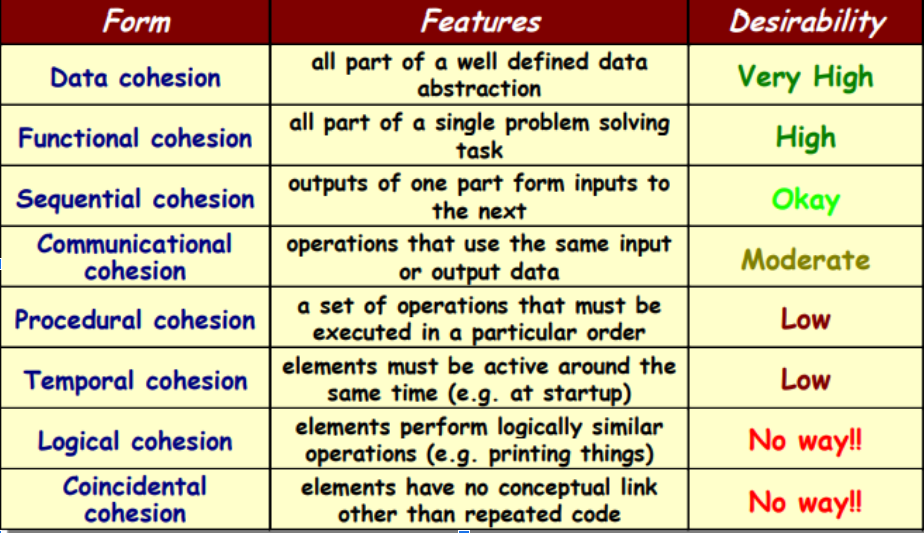
\includegraphics[scale=0.4]{figs/cohesion.png}
	\caption{انواع cohesion}	
	\label{farzamfig2}
\end{figure}

برای آنکه در حین طراحی به کیفیت هم توجه داشته باشید راهنمایی‌هایی داریم که در اسلاید‌های درس به آن‌ها اشاره شده و در اینجا اشاره‌ دوباره‌ای به آن‌ها نخواهیم کرد چرا که هدفمان بررسی کیفیت طراحی است.

به طور کلی ۴ معیار کلیدی برای بررسی کیفیت موارد زیر هستند:
قابلیت اطمینان، بهره وری، قابلیت نگهداری و قابلیت استفاده.

{\Large پیش‌بینی‌های قابل اندازه‌گیری راجع به کیفیت}

{\large \textbf{سادگی} (simplicity)}

یعنی طراحی اهداف مورد نظر را برآورده کند و کارهای اضافه‌ی دیگری را در خود نداشته باشد. برای اندازه‌گیری و بررسی آن می‌توان از روش‌های زیر استفاده کرد:
\begin{enumerate}
	\item بررسی پیچیدگی جریان کنترل (برای مثال تعداد مسیرهای گراف جریان کنترل)
	\item بررسی پیچیدگی جریان اطلاعات (برای مثال تعداد داده‌های مشترک)
	\item بررسی پیچیدگی فضای نام‌ها (برای مثال بررسی تعداد عملوند‌ها و عملگرها)
\end{enumerate}


{\large \textbf{ماژول‌ماژول بودن} (modularity)}

نگرانی‌های مختلف داخل طراحی از هم جدا شده باشند. برای بررسی این منظور هم  به بررسی cohesion و coupling می‌پردازیم.


\subsection*{مراجع}

\begin{latin}
	\begingroup
	\renewcommand{\section}[2]{}%
	
\begin{thebibliography}{9}
%   Check this for adding items: https://www.student.unsw.edu.au/how-do-i-cite-electronic-sources	
	\bibitem{Budgen, 1994}
	\textit{Budgen, D. “Software Design”, 1994, pp65-7}
	
	\bibitem{Toronto slides}
	\textit{\url{http://www.cs.toronto.edu/~sme/CSC444F/slides/L12-SoftwareQuality.pdf}}

\end{thebibliography}
\endgroup
\end{latin}

}
